\section{收敛与计算成本}
\label{sec:fom-cost}

前三节各自给出了保证和例子。于是要问：要在几种方法中选择时，应该按什么标准比较？按第~\ref{chap:smooth-foundations}章的约定，比较时要固定三件事：度量误差的量、停止精度和要报告的迭代点，然后计算达到这一精度所需的总计算。

\paragraph{同样的尺子}
贯穿例上，以梯度大小不超过$10^{-3}$为停止标准，各方法的结果如下表。固定步长的方法每步读一次梯度，读取次数与步数大体相等。

\begin{BookInlineTable}
  \centering
  \caption{贯穿例上达到$\lVert\bm{g}\rVert_2\leq10^{-3}$的步数。}
  \label{tab:fom-example-count}
  \begin{tabular}{lll}
   \toprule
   方法 & 参数 & 步数\\
   \midrule
   梯度下降 & $\alpha=1/9$ & $78$\\
   梯度下降 & $\alpha=1/5$ & $43$\\
   重球法 & $\alpha=\beta=1/4$ & $19$\\
   Nesterov方法 & $\alpha=1/9$，$\beta=1/2$ & $29$\\
   共轭梯度 & 精确线搜索 & $2$\\
   \bottomrule
  \end{tabular}
\end{BookInlineTable}

这张表不能拿来宣布胜负。共轭梯度的$2$步依赖于目标是二次的，而且精确步长用到了$\bm{H}$；重球法的$19$步依赖于事先知道$\mu$和$L$，并且只对二次目标有理论保证；三种固定步长的方法都不必做线搜索。下面把这些差异分别计入。

\paragraph{保证的比较}
下表汇总本章的保证，$R=\lVert\bm{x}^{(0)}-\bm{x}^\star\rVert_2$，$\Delta=f(\bm{x}^{(0)})-f_{\inf}$。不同列的度量不同：非凸列是梯度大小，凸与强凸列是目标差。

\begin{BookInlineTable}
  \centering
  \caption{各方法的理论保证，$\Phi^{(0)}=f(\bm{x}^{(0)})-f^\star+\tfrac\mu2R^2$，“—”表示本章不给结论。}
  \label{tab:fom-guarantees}
  \begin{tabular}{llll}
   \toprule
   方法 & 非凸 & 凸 & 强凸\\
   \midrule
   梯度下降 & $\min\lVert\bm{g}\rVert_2^2\leq\frac{2L\Delta}{T}$ & $\frac{LR^2}{2T}$ & $(1-\frac1\kappa)^T\Delta$\\
   重球法 & — & — & 二次目标$(2T+1)\rho^T$\\
   Nesterov方法 & — & $\frac{2LR^2}{(T+1)^2}$ & $(1-\frac{1}{\sqrt\kappa})^T\Phi^{(0)}$\\
   FR & $\liminf\lVert\bm{g}\rVert_2=0$ & 同左 & 同左\\
   \bottomrule
  \end{tabular}
\end{BookInlineTable}

重球法一行的界是解距离的比例，$\rho=(\sqrt\kappa-1)/(\sqrt\kappa+1)$。FR的“同左”表示在凸和强凸情形下，本章的定理仍然只给出驻点型的结论。这与实际的快慢不是一回事：FR在实践中常比梯度下降快，但本章的定理没有给出这一点。

$T$与$\kappa$的影响可以换算成具体的数字。取$\kappa=10^4$，目标差要降到初值的$10^{-6}$，$\ln10^6\approx13.8$，于是
\[
 \kappa\ln\frac1\varepsilon\approx1.38\times10^5,\qquad
 \sqrt\kappa\ln\frac1\varepsilon\approx1.38\times10^3.
\]

相差一百倍。这是梯度下降与加速方法在定理的上界上的差别。Nesterov方法的$\sqrt\kappa$和$1/T^2$依赖，在“新迭代点只在已读取梯度的张成空间内”这类方法中不能进一步改进；证明需要构造一个三对角的二次函数，让前$T$步的梯度只能探到前$T$个坐标，篇幅较长，读者可查阅凸优化的专门著作。图~\ref{fig:fom-nag-convex}所用的函数正是这种构造。

\paragraph{一步要花多少}
迭代次数只是总计算的一个因子。每步的代价由三部分构成：梯度读取、线搜索的函数试探、向量的更新与存储。

\begin{BookInlineTable}
  \centering
  \caption{每步的代价，维数为$n$。}
  \label{tab:fom-cost-per-step}
  \begin{tabular}{llll}
   \toprule
   方法 & 梯度读取 & 存储向量 & 需要的信息\\
   \midrule
   梯度下降（固定） & $1$ & $2$ & $L$\\
   梯度下降（回溯） & $1$加试探 & $2$ & 无\\
   重球法 & $1$ & $3$ & $L,\mu$\\
   Nesterov方法 & $1$ & $3$ & $L$，强凸时加$\mu$\\
   非线性共轭梯度 & 多次 & $3$到$4$ & 无\\
   \bottomrule
  \end{tabular}
\end{BookInlineTable}

向量更新都是$O(n)$，与读一次梯度相比通常可以忽略。除非目标是高度结构化的，读一次梯度的代价要大得多。所以比较的主要量是梯度与函数的读取次数，而不是迭代步数。

强Wolfe线搜索每步要在试探点上计算函数值和方向导数，后者需要整个梯度，一次试探大约相当于一次完整的梯度读取。试探次数取决于初始步长的猜测和$c_2$的松紧。例如弯谷上$c_2=0.4$时，PRP+走了$24$步，用了$75$次读取，平均每步约$3$次。

\paragraph{步数少不等于计算少}
图~\ref{fig:fom-cost}在一个$100$维的问题上比较四种方法：
\[
 f(\bm{x})=\frac12\sum_{i=1}^{100}\lambda_ix_i^2+\sum_{i=1}^{100}\ln\cosh x_i,
\]
其中$\lambda_i$在$[1,1000]$内按对数等距分布。目标强凸，$\mu=1$，$L=1001$，要求$\lVert\bm{g}\rVert_2\leq10^{-6}$。

\begin{BookInlineFigure}
  \centering
  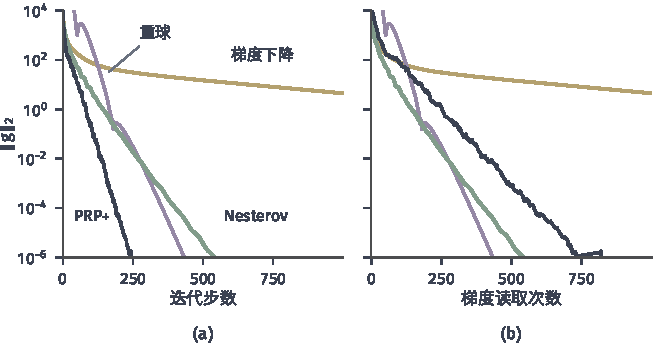
\includegraphics[width=112mm]{figures/05-optimization/02-smooth-optimization/matplotlib/fom-cost/figure.pdf}
  \caption{$100$维强凸非二次目标上的梯度大小，$\kappa=1001$，起点由固定种子的正态随机数给出。黄线是$\alpha=1/L$的梯度下降，紫线是按式~\eqref{eq:fom-hb-params}取参数的重球法，绿线是强凸参数的Nesterov方法，黑线是PRP+配合强Wolfe线搜索（$c_1=10^{-4}$，$c_2=0.1$）。(a)横轴是迭代步数。(b)横轴是梯度读取次数，同一组数据的位置变了。}
  \label{fig:fom-cost}
\end{BookInlineFigure}

按迭代步数，PRP+最少，$244$步，重球法$434$步，Nesterov方法$542$步，梯度下降$7574$步。按梯度读取，PRP+用了$821$次，比重球法的$435$次和Nesterov方法的$543$次都多。只看左图会选PRP+，只看右图会选重球法。

这张图也提醒另一点。重球法在这里表现好，但定理不保证它：目标不是二次的。Nesterov方法多读了约百分之二十五的梯度，换来的是对这一类目标有定理保证。四种配置中只有PRP+不需要$L$和$\mu$。这两个常数无法估计时，它可以直接运行；梯度下降配回溯也能做到这一点，只是更慢。

\paragraph{输出什么}
最后要说明报告哪个点。按定理~\ref{thm:fom-gd-nonconvex}的说法，非凸时应记录梯度最小的迭代点；凸与强凸的定理针对最后一个迭代点。Nesterov方法的目标差不单调，如果需要，可以另外保留函数值最低的点，这只需要在已经计算函数值时比较。

非线性共轭梯度的$\liminf$结论并不保证最后一点最好，同样应保留历史最优点。无论哪种方法，宣布达到精度之前都应该在输出点处重新计算一次梯度，而不是用外推点的梯度代替，后者并不是输出点的残差。
